\section{Μοντέλο Οντοτήτων/Συσχετίσεων}

\subsection{Γενική Περιγραφή}

\{Αναφέρετε συνοπτικά ποιες είναι οι οντότητες του συστήματός σας και
πως συνδέονται. Σε αυτό το σημείο μην ξεχάσετε να αναφέρετε όλες τις
υποθέσεις στις οποίες βασίζεστε.\}

Παράδειγμα για τη FlightsDB:

Οι οντότητες είναι η Πτήση (FlightInstance), το Αεροδρόμιο (Airport),
κτλ. Για κάθε πτήση θα πρέπει να καταγράφεται ένα αεροδρόμιο
αναχώρησης και ένα αεροδρόμιο προορισμού…

Υποθέσεις:
\begin{itemize}[noitemsep]
\item Ο κωδικός πτήσης είναι μοναδικός για κάθε ημέρα. Για παράδειγμα,
  εφόσον ο κωδικός 101 αντιστοιχεί σε μια συγκεκριμένη πτήση (ασχέτως
  αεροδρομίων) την ημερομηνία 27/12/2018, τότε ο ίδιος κωδικός (101)
  δε μπορεί να είναι ο κωδικός καμίας άλλης πτήσης.
\item \ldots
\end{itemize}

\subsection{Καθορισμός Οντοτήτων}

\{Αναφέρετε τις οντότητες της βάσης δεδομένων, καθώς και τα γνωρίσματά
τους.\}

Παράδειγμα για τη FlightsDB:

\begin{tabular}{|l|l|l|}
  \hline
  \textbf{Όνομα Οντότητας} &\multicolumn{2}{|l|}{Airport}\\ \hline
  \textbf{Περιγραφή}&\multicolumn{2}{|l|}{Οντότητα που αποθηκεύονται τα αεροδρόμια}\\ \hline
  \textbf{Ιδιότητες}&\multicolumn{2}{|l|}{Ισχυρή Οντότητα, \ldots \{αναφέρετε επίσης υπο/υπερκλάσεις\}}\\ \hline
  \textbf{Γνωρίσματα}&\multicolumn{2}{|l|}{airport\_code} \\ \cline{2-3}
                          &\multicolumn{2}{|l|}{airport\_name}\\
  \cline{2-3}
                           &airport\_address <σύνθετο>&street \\
  \cline{3-3}
                           &&city \\ \cline{3-3}
                           &&zip \\ \hline
\end{tabular}

\subsection{Καθορισμός Συσχετίσεων}

/{Αναφέρετε τις συσχετίσεις της βάσης δεδομένων./}

Παράδειγμα για τη FlightsDB:

\begin{tabular}[]{|p{4cm}|p{10cm}|}
  \hline
  \textbf{Όνομα Συσχέτισης} & Flight\_Has\_Airport \\ \hline
  \textbf{Περιγραφή} & Κάθε πτήση πρέπει να έχει ένα αεροδρόμιο
                       αναχώρησης και ένα αεροδρόμιο προορισμού \\ \hline
  \textbf{Ιδιότητες} & Has-A \{αναφέρετε αν είναι Is-A και αν είναι
                       Αναδρομική, Προσδιορίζουσα, Τριαδική\} \\ \hline
  \textbf{Λόγος πληθικότητας} & 1:2 \\ \hline
  \textbf{Συμμετοχή} & Ολική Συμμετοχή του Flight \\ \cline{2-2}
                            &Συμμετοχή του Airport \\ \hline
  \textbf{Γνωρίσματα} & - \\ \hline
\end{tabular}

\subsection{Διάγραμμα Οντοτήτων/Συσχετίσεων}

\{Δείξτε το διάγραμμα Ο/Σ για τη βάση. Το διάγραμμα μπορείτε να το
κατασκευάσετε σε πρόγραμμα της επιλογής σας, ωστόσο θα πρέπει να
ακολουθεί το συμβολισμό Chen (δηλαδή οντότητες ως παραλληλόγραμμα,
συσχετίσεις ως ρόμβοι, διπλή γραμμή για υποχρεωτική συμμετοχή, κτλ.)\}

Παράδειγμα για τη FlightsDB:
\begin{figure}[H]
  \centering
  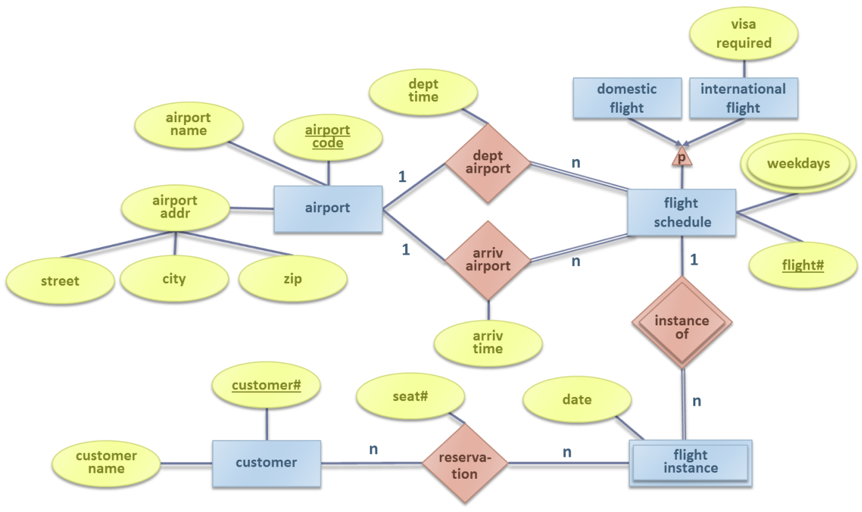
\includegraphics[width=\linewidth]{entities.png}
  \caption{Διάγραμμα Οντοτήτων/Συσχετίσεων}
\end{figure}


%%% Local Variables:
%%% mode: latex
%%% TeX-master: "main"
%%% End:
